%%
%% This is file `sample-sigconf.tex',
%% generated with the docstrip utility.
%%
%% The original source files were:
%%
%% samples.dtx  (with options: `sigconf')
%% 
%% IMPORTANT NOTICE:
%% 
%% For the copyright see the source file.
%% 
%% Any modified versions of this file must be renamed
%% with new filenames distinct from sample-sigconf.tex.
%% 
%% For distribution of the original source see the terms
%% for copying and modification in the file samples.dtx.
%% 
%% This generated file may be distributed as long as the
%% original source files, as listed above, are part of the
%% same distribution. (The sources need not necessarily be
%% in the same archive or directory.)
%%
%% The first command in your LaTeX source must be the \documentclass command.
\documentclass[sigconf]{acmart}

%%
%% \BibTeX command to typeset BibTeX logo in the docs
\AtBeginDocument{%
	\providecommand\BibTeX{{%
			\normalfont B\kern-0.5em{\scshape i\kern-0.25em b}\kern-0.8em\TeX}}}

%% Rights management information.  This information is sent to you
%% when you complete the rights form.  These commands have SAMPLE
%% values in them; it is your responsibility as an author to replace
%% the commands and values with those provided to you when you
%% complete the rights form.
\setcopyright{none}
%\setcopyright{acmcopyright}
%\copyrightyear{2018}
%\acmYear{2018}
%\acmDOI{10.1145/1122445.1122456}

%% These commands are for a PROCEEDINGS abstract or paper.
%\acmConference[Woodstock '18]{Woodstock '18: ACM Symposium on Neural Gaze Detection}{June 03--05, 2018}{Woodstock, NY}
%\acmBooktitle{Woodstock '18: ACM Symposium on Neural Gaze Detection, June 03--05, 2018, Woodstock, NY}
%\acmPrice{15.00}
%\acmISBN{978-1-4503-9999-9/18/06}


%%
%% Submission ID.
%% Use this when submitting an article to a sponsored event. You'll
%% receive a unique submission ID from the organizers
%% of the event, and this ID should be used as the parameter to this command.
%\acmSubmissionID{123-A56-BU3}

%%
%% The majority of ACM publications use numbered citations and
%% references.  The command \citestyle{authoryear} switches to the
%% "author year" style.
%%
%% If you are preparing content for an event
%% sponsored by ACM SIGGRAPH, you must use the "author year" style of
%% citations and references.
%% Uncommenting
%% the next command will enable that style.
%%\citestyle{acmauthoryear}

%%
%% end of the preamble, start of the body of the document source.

\usepackage{CJKutf8}
\usepackage{diagbox}
\usepackage{multirow}
\usepackage{amsthm}
\usepackage{mathtools}
\usepackage{hhline}
\usepackage{booktabs}

\newcommand{\JQ}[1]{\textcolor{blue}{JQ: #1}}
\newcommand{\KZ}[1]{\textcolor{red}{Kenny: #1}}


\begin{document}
	\fancyhead{}
	%%
	%% The "title" command has an optional parameter,
	%% allowing the author to define a "short title" to be used in page headers.
	\title{CoCon: A Dataset of Commonsense Contradiction on Short Phrase Constructed from the Web}
	
	%%
	%% The "author" command and its associated commands are used to define
	%% the authors and their affiliations.
	%% Of note is the shared affiliation of the first two authors, and the
	%% "authornote" and "authornotemark" commands
	%% used to denote shared contribution to the research.
	%\author{Ben Trovato}
	%\authornote{Both authors contributed equally to this research.}
	%\email{trovato@corporation.com}
	%\orcid{1234-5678-9012}
	%\author{G.K.M. Tobin}
	%\authornotemark[1]
	%\email{webmaster@marysville-ohio.com}
	%\affiliation{%
	%	\institution{Institute for Clarity in Documentation}
	%	\streetaddress{P.O. Box 1212}
	%	\city{Dublin}
	%	\state{Ohio}
	%	\postcode{43017-6221}
	%}

	
	%%
	%% By default, the full list of authors will be used in the page
	%% headers. Often, this list is too long, and will overlap
	%% other information printed in the page headers. This command allows
	%% the author to define a more concise list
	%% of authors' names for this purpose.
	\renewcommand{\shortauthors}{Trovato and Tobin, et al.}
	
	%%
	%% The abstract is a short summary of the work to be presented in the
	%% article.
	\begin{abstract}
		Commonsense knowledge consists of short and simple concepts about the everyday life such as ``blue sky'' instead of ``green sky'', which all humans agree with.
		Incorporating commonsense knowledge to machines is a long-standing challenge to fulfill real artificial intelligence.
		Unlike previous work mainly focusing on inferences between long sentences, we target on short phrase pairs, which is more challenging for a lack of surrounding context. 
		With the help of our constructed \textit{Concept Association Graph} which contains abundant web knowledge, 
		we propose a new dataset \textbf{CoCon} with over 9,000 pairs of short phrases extracted from web queries, which is designed for testing the capability of machines on commonsense reasoning.
%\KZ{I suggest we rename the dataset to CoCon, to avoid confusion with MS Coco and also
%contradiction should be simplified to con rather than co.}
		Preliminary experiments show that large pre-trained language models such as BERT and ERNIE are still lagging behind human performance by a large margin on CoCon, which indicates that further efforts are needed to enable machines to grasp such commonsense knowledge. 
%\KZ{I don't quite see this paper's relevance to the Web! This should be stressed both
%in abstract and in the intro.}
	\end{abstract}
	
	%%
	%% The code below is generated by the tool at http://dl.acm.org/ccs.cfm.
	%% Please copy and paste the code instead of the example below.
	%%
	%\begin{CCSXML}
	%	<ccs2012>
	%	<concept>
	%	<concept_id>10010520.10010553.10010562</concept_id>
	%	<concept_desc>Computer systems organization~Embedded systems</concept_desc>
	%	<concept_significance>500</concept_significance>
	%	</concept>
	%	<concept>
	%	<concept_id>10010520.10010575.10010755</concept_id>
	%	<concept_desc>Computer systems organization~Redundancy</concept_desc>
	%	<concept_significance>300</concept_significance>
	%	</concept>
	%	<concept>
	%	<concept_id>10010520.10010553.10010554</concept_id>
	%	<concept_desc>Computer systems organization~Robotics</concept_desc>
	%	<concept_significance>100</concept_significance>
	%	</concept>
	%	<concept>
	%	<concept_id>10003033.10003083.10003095</concept_id>
	%	<concept_desc>Networks~Network reliability</concept_desc>
	%	<concept_significance>100</concept_significance>
	%	</concept>
	%	</ccs2012>
	%\end{CCSXML}
	
	%\ccsdesc[500]{Computer systems organization~Embedded systems}
	%\ccsdesc[300]{Computer systems organization~Redundancy}
	%\ccsdesc{Computer systems organization~Robotics}
	%\ccsdesc[100]{Networks~Network reliability}
	
	%%
	%% Keywords. The author(s) should pick words that accurately describe
	%% the work being presented. Separate the keywords with commas.
	\keywords{datasets, commonsense, E-commerce}
	
	%% A "teaser" image appears between the author and affiliation
	%% information and the body of the document, and typically spans the
	%% page.
	
	
	%%
	%% This command processes the author and affiliation and title
	%% information and builds the first part of the formatted document.
	\maketitle
	
	\begin{CJK}{UTF8}{gbsn}
	\section{Introduction}

Protein$-$protein interactions (PPIs) are of central importance for the majority of biological functions, such as signal transduction, metabolic pathways, molecular dynamics, and protein networks\cite{Hoffmann.Krallinger.ea:2005}, for they serve as the most fundamental building blocks of the entire interacademic systems of any organisms. Collecting data on pairwise interaction relationships is essential for multiple purpose, including identification of modules with certain functionality\cite{Spirin.Mirny.03}, mapping diseases to dominated genes\cite{Ideker.Sharan.08}, and after all, understanding wholistic metabolic/genetic networks from a system biology perspective.

A lot of databases have been built to store protein and genetic interactions from major model organism species and are available in various standardized formats, such as MINT\cite{Zanzoni.Montecchi-Palazzi.ea:2002}, BIND\cite{Bader.ea:2003}, BIOGRID\cite{DBLP:journals/nar/StarkBRBBT06}, etc. Among those mainstream databases, the data largely rely on voluntary reports by scientists or researchers, besides, comprehensive curation efforts become indispensable for the sake of accuracy. However, the amount of biology-related literatures with respect to protein interactions grows explosively and thus make it either impossible or impractical to manually detect PPI information anymore.

Considering huge amount of PPI information with great wealth hidden in published papers, in recent years, numerous mining techniques have been proposed that aim to extract PPI information automatically from free text, especially machine learning, information retrieval, and natural language processing\cite{DBLP:journals/bib/WinnenburgWPDS08}.These approaches can be roughly categorized into three classes: co$-$occurrence, rule$-$based, and machine learning. 

Co$-$occurrence is the approach with most simplicity and naivete. Just as its name implies, this method intends to find out pairs of proteins that co-occur in the same context. The scope of "same context" ranges from phrase, sentence, paragraph to whole abstract, even document. The underlying assumption is that whenever two proteins are mentioned together by authors, chances are high that there is some kind of relationship between them. However, however, in-context closeness even semantic relation does not necessarily represent actual biological interaction. As a consequence, a large fraction of candidate pairs are mismatched inevitably, causing a high recall but low precision.

The second approach is rule-based extraction, in other words, pattern matching. There are many types of rules, most of them concern natural language processing (NLP). One way is to specify hand-crafted regular expressions before hand, which mostly lean on language usage preference. Besides, by using full or partial (shallow) parsing strategies, more information would be acquired, such as part-of-speech taggers, local dependencies between syntactic components, context-free grammar\cite{DBLP:journals/bioinformatics/TemkinG03}, and full sentence structure. Compared to co$-$occurrence, rule-based approach enjoy better precision but much lower recall. In addition, since the rules are usually derived from training data, that is to say, the improper choice of training data would be significantly lethal, therefore quality of extraction is invariably instable and may not applicable to other data.

The third and most commonly used approach use machine learning techniques, in this case, the task to extract protein$-$protein interactions turns out to be a binary classification problem. Each protein pairs are represented along with a set of features, which is associated with their context, then a well$-$defined classifier gives the answer whether the candidate protein pairs is classified to be qualified PPI. (TO BE FURTHER FILLED!!!)

In this paper, we introduce a general bootstrapping framework for Protein$-$protein interaction extraction from natural text.Our method differs from most of the previous works in three aspects:

(1)The extraction process is driven by only tiny fraction of training data, which are regarded as seed data. In each round, it would derive reliable patterns automatically from seed data, then extract more positive PPI pairs consequently, what's more, the seed data would be augmented by the newly extracted results with high confidence.

(2)multiple graph kernel. 

(3)various evaluation.




	\section{Related Work}
This section surveys previous works on question generation and tree encoding
respectively.

Text question generation has attracted the attention 
after the work of ~\citeauthor{du2017learning}~\shortcite{du2017learning}, who uses deep seq2seq model 
to generate questions from a raw text paragraph. 
Before that, text question generation relied heavily on hand-craft 
question patterns~\cite{HeilmanS10,LabutovBV15,MostowC09} which is time and 
labor consuming. 

However, this pure seq2seq model is not focused and 
has no control over part in the paragraph to generate question. 
~\citeauthor{zhou2017neural}~\shortcite{zhou2017neural} proposed to encode 
key phrase information using binary indicators to generate 
key-aware questions and they assumes the answer to be key phrase. 
Considering key phrase (answer) is unavailable in reality, 
~\citeauthor{SubramanianWYT17}~\shortcite{SubramanianWYT17} applied 
a two-stage approach. First, key phrases are extracted by 
pointer network~\cite{ptrnet}. Second, 
key phrases are encoded in the same way as 
Zhou et al. With the intuition that questions could be asked in many ways, 
~\citeauthor{Yao2018vae}~\shortcite{Yao2018vae} used conditional-VAE to 
increase the diversity of questions. More recently, models with 
auxiliary feature information~\cite{HarrisonW18} helped improve 
the question quality. Structure question generation aims at 
converting structured data such as triples in knowledge graph to questions. 
~\citeauthor{SerbanGGACCB16}~\shortcite{SerbanGGACCB16} proposed a model to generate factoid questions from knowledge base triples.  None of the above work
considered using parse tree structures to aid question generation process,
which is the focus of this paper.

Sequential RNN model takes sentence as a sequence of words, 
ignoring the syntactic information. In order to utilize
such syntactic information with sequential information, 
~\citeauthor{tai2015improved}~\shortcite{tai2015improved} proposed Tree-LSTM to 
encode the binary parse tree recursively in a bottom-up fashion to 
classify sentiment. In text generation task, 
\citeauthor{eriguchi2016tree}~\shortcite{eriguchi2016tree} 
proposed a tree-to-sequence model with attention mechanism to do 
machine translation and 
~\citeauthor{liang2018automatic}~\shortcite{liang2018automatic} proposed a 
tree-to-sequence model which could handle arbitrary trees, 
to do code comment generation. Our work is inspired by these previous
attempts and we are first to adapt structure encoded neural models to
textual question generations.
	\section{CoCon Dataset}
\label{sec:cocon}
In this section, we first present our dataset form. Next, we describe data collection process, including text crawling, phrase pre-selecting, annotation, auto-generation and quality control. To better understand our CoCon dataset, we also conduct an analysis on the characteristics of all samples. The dataset collection process is shown in Figure~\ref{fig:framework}. Although the proposed dataset is in Chinese, the methodology can be easily extended to other languages.

\begin{figure}
	\centering
	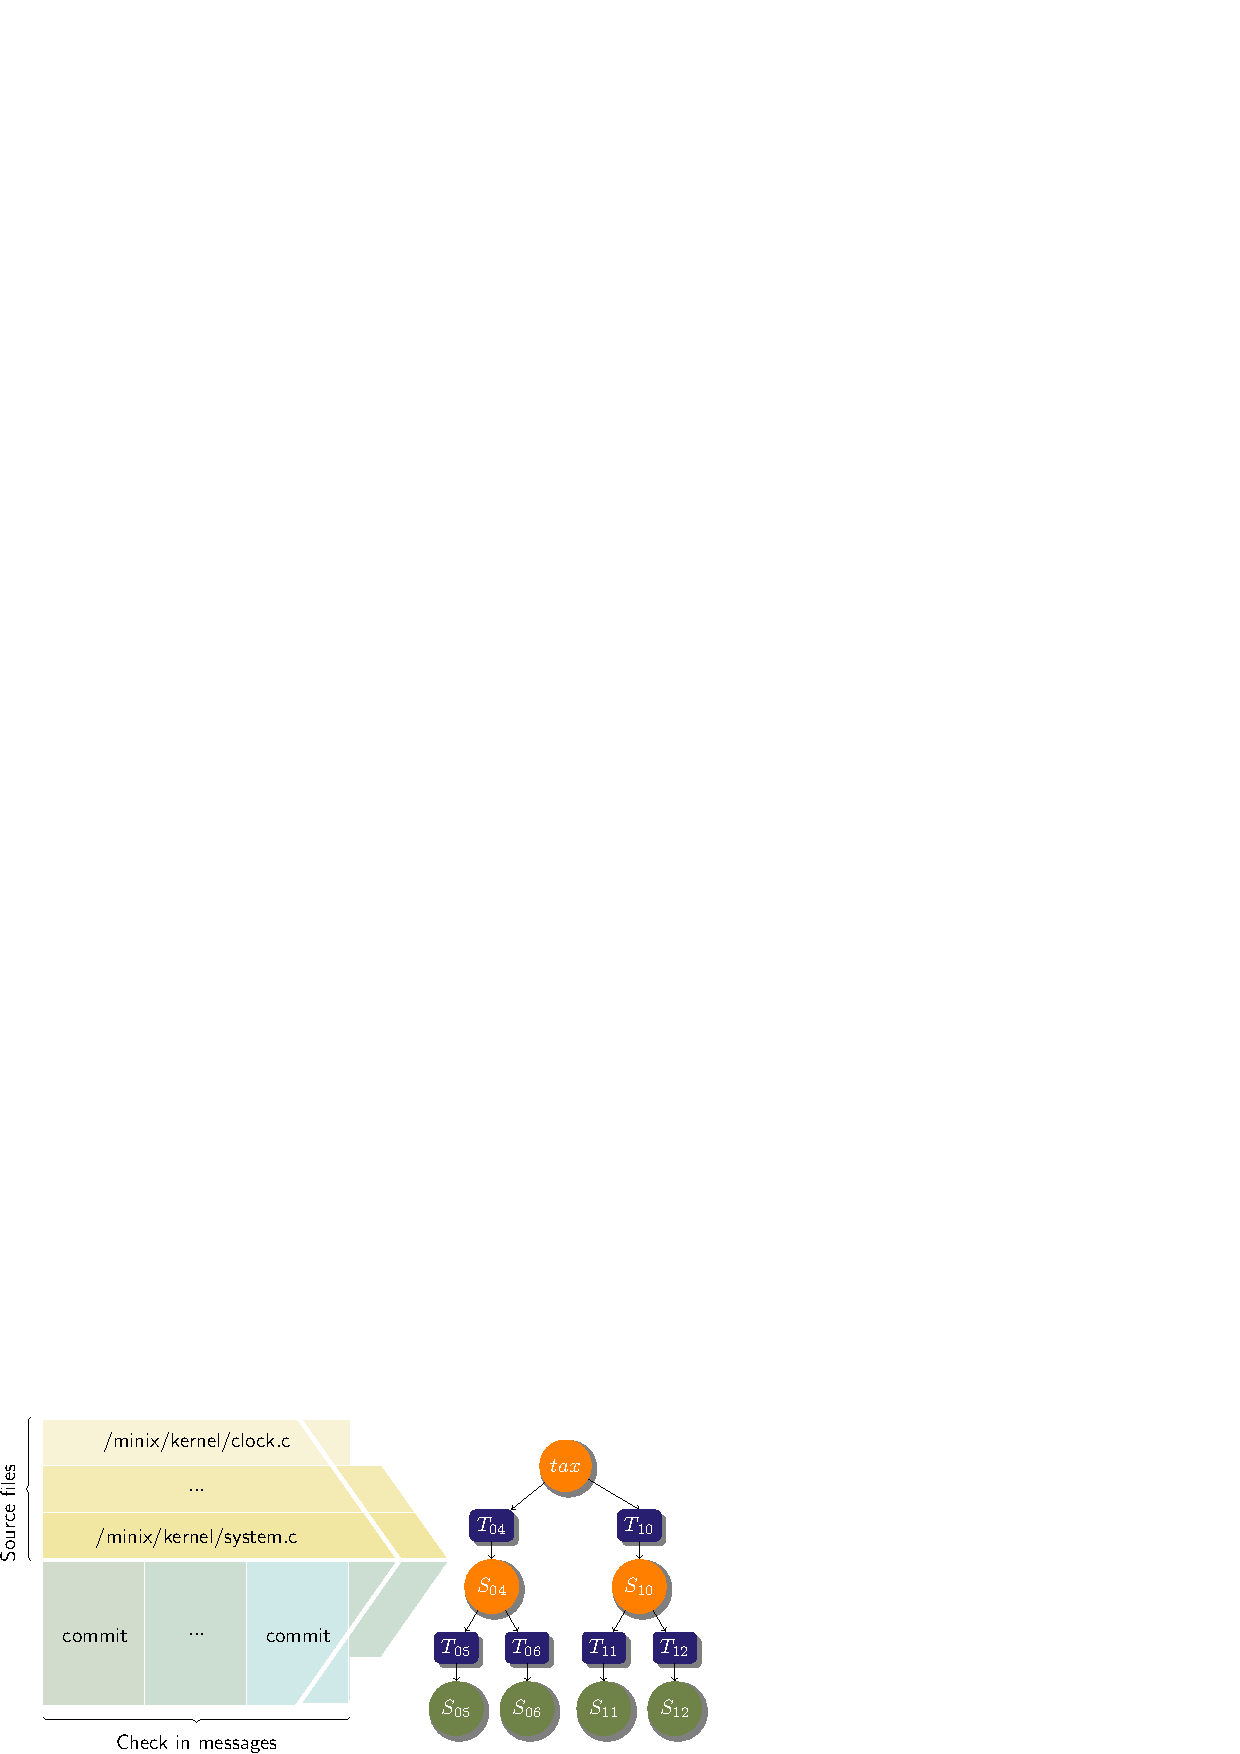
\includegraphics[width=\columnwidth]{images/framework.pdf}
	\caption{CoCon dataset collection process}
	\label{fig:framework}
\end{figure}

\subsection{Dataset Introduction}
Each instance in our CoCon dataset is a triple: $\{p_1, p_2, l\}$, where $p_1$ and $p_2$ are two similar phrases sharing most words, focusing on the same subject
but with different modifiers.
%However, only one of them is plausible by common sense. 
$l$ is the label which indicates the index of the more plausible phrase. 
Therefore, the whole task can be seen as a binary classification problem 
and we use accuracy as evaluation metric. 

In our problem, instead of judging if one phrase is plausible, a pair of phrases are offered to be compared. This is based on that common sense has no absolute criteria. 
Neither can we simply select a threshold for a model to give answer. Hence, we design the task as comparison problem.
%the task as a question of comparison.

\subsection{Raw Data Preprocessing}
%We crawl search queries from a popular e-commerce platform 
%where some noisy and meaningless queries are filtered
%through query normalization including lexical error corrections and query rewriting.

We crawl search queries from a popular Chinese E-commerce platform\footnote{https://www.taobao.com/} and compute lexical and grammatical error corrections using pre-trained neural network. 
We further filter out queries including numbers and English chararacters keeping
those queries composed of only Chinese characters. 
At this point, 4,081,254 common queries remain. 
The length of these queries ranges from 2 to 15, and is 4.73 on average. 
The number of words\footnote{Word segmentations are done by using tools trained 
on E-commerce data in advance.} in queries is distributed between 2 to 8 and 2.07 
on average. 
%The details of character and word number distribution is shown in Figure \ref{fig:wordDist}. 

%\begin{figure}
%	\centering
%	\includegraphics[width=0.95\columnwidth]{images/distributionWords.pdf}
%	\caption{Char and word number distribution of raw data after preprocessing}
%	\label{fig:wordDist}
%\end{figure}


%\subsection{Preprocessed Data Overview}
\subsection{Auto-generation of CoCon pairs}
We define phrases that have commonsense contradiction as \textit{positive samples}, such as ``children's sexy dress" and other phrases as \textit{negative samples} such as ``children's blue dress". 

To have a preliminary and rough understanding over the raw dataset
, we first randomly select 10,000 phrases from preprocessed raw data and do the human annotation. 
Among all selected samples, we find 292 positive samples and 9708 negative samples. It should be noticed that positive samples are much rarer than negative ones, only account for 2.92\%. Obviously, directly annotating the original collection of queries to get more positive samples is not efficient.
%Therefore, we come up with two methods to get expected phrase pairs in CoCon dataset more efficiently: \textbf{Random Replacement} and \textbf{Filter using graph}.
%Therefore, we come up with a method called \textbf{filter using graph} to get expected phrase pairs more efficiently. 


The main idea is that a popular query is more likely to be plausible. 
We propose to construct \textit{Concept Association Graph}, weighted with co-occurrences in the same query between terms by using a large user queries corpus.

%\textit{Step 1: Positive samples preselecting}
\subsubsection{Positive samples preselecting}
%We first crawled user queries on e-commerce platform with data masking among 7 days (2019.07.15-2019.07.21).
We first crawled user queries during 7 days (2019.07.15-2019.07.21) on E-commerce platform after data masking. 
There are 303,285,752 legitimate queries (all Chinese characters with at least
one word) in all. Then we analyze each query to get co-occurrence of each word pair, 
and gradually enrich the graph.
For example, from the query ``sexy blue dress'', we will get three word pairs 
(sexy, dress), (blue, dress) and (sexy, blue). Notice that the edge in our net does not have directions and the word order is neglected.
% in word pairs is of no importance.
Besides, word synonyms are combined together using a Chinese synonym dictionary provided by HIT-SCIR\footnote{https://ltp-cloud.com/download/}.
After construction, the weight of each edge in the graph represents the frequency 
that this word pair was observed in the whole user query corpus. 
A fragment of our constructed \textit{Concept Association Graph} is shown in Figure \ref{fig:net}.

\begin{figure}
	\centering
	\includegraphics[width=0.8\columnwidth]{images/associationNetColor.pdf}
	\caption{A fragment of \textit{Concept Association Graph}}
	\label{fig:net}
\end{figure}

However, the non-uniform user distribution can lead to bias. For example, there may
be more female users than male users. As a result, the frequency of word pair 
(electric, dress) may larger than that of (electric, torch) even though the former
is less plausible.

Mutual information is a suitable criterion to measure the dependency of two words. 
If word A appears $x$ times in the query corpus, word B appears $y$ times, 
the word pair (A,B) appears $z$ times, and the total number of words is $N$, then the mutual information between word A and B is defined as:
\begin{equation}
I(A,B) = log\frac{P_r(A\wedge B)}{P_r(A)\times P_r(B)}
\end{equation}
and can be estimated as:%using:
\begin{equation}
I(A,B) \approx log\frac{z\times N}{(x+z)\times (y+z)}
\end{equation}

We use mutual information to calculate the strength of word associations in 
our constructed graph, which is noted as ``plausibility.''
For a phrase $T=(w_1, ..., w_m)$, %there may be not only two words, 
where there is more than two words, 
we calculate the overall plausibility $P$ as:
\begin{equation}
P(T) = \frac{2}{m*(m-1)}\sum_{i=1}^{m-1}\sum_{j=i+1}^{m}I(w_i, w_j)
\end{equation}

Besides, based on the idea that phrases should be common enough,
we remove the phrase which contains any rare word that appears less than a threshold in our graph.
1 million is set as threshold in our problem as total number of queries are more than 300 millions.   %\KZ{100,000 seems like a very large number!}
%If all word pairs in a phrase doesn't exist in our graph, this phrase will also be filtered. Then, 
The remained phrases are ranked according to their overall plausibility score from small to large to get the most implausible phrase list.

To evaluate the effectiveness of the above method, we test on our 10,000 preliminary annotated phrases. %as example.
After removing rare words, 6,381 phrases (include 94 positive ones) are removed where the rate of positive phrase is 1.47\%. After removing non-exist word pair, another 107 phrases (include 9 positive ones) are removed. Finally, 3,512 phrases (include 167 positive ones) remain. Among top 526 phrases (15\%), 77 positive ones are found, where the rate of positive phrases achieves 15.4\%, %remarkably increases compared to 2.92\% on randomly selected raw data.
achieves a remarkable increase from 2.92\% on randomly selected raw data.
%on the 10,000 randomly selected on preprocessed raw data.
%showing the validity of the constructed graph.

%Therefore, we apply 
Verifying the validity of \textit{Concept Association Graph}, the above method is applied on 
our whole unlabeled preprocessed 4,081,254 phrases,
%top 15\% (1,176,922 phrases) of overall plausibility score are kept. 
we fetch the top 18,000 phrases which have low plausibility score for human annotation due to the 
limited resources.

%\textit{Step 2: Phrase Annotation}
\subsubsection{Phrase Annotation}

This part describes the guideline for annotators: when to ignore a phrase and what kind of implausible phrases do we need.
\begin{enumerate}
	\item Phrases that belong to any one of these three cases can be directly ignored: 
	\begin{itemize}
		\item [-] Plausible phrase.
		\item [-] Absence of a clear subject.
		\item [-] Contains rare word~(i.e., unfamiliar to the annotator)
	\end{itemize}
	\item Judge the phrase to be implausible if it belongs to the following four commonsense contradiction category:
	\begin{itemize}
		\item [-] Several modifiers are contradictory between themselves. %Several modifiers for one subject and commonsense contradiction exists between modifiers. 
		For example, in ``Europe Korean curtain''~(欧韩窗帘), two national modifiers are contradictory.
		
		\item [-] The modifier is contradictory with the intrinsic property of subject. For example, ``vitreous porcelain''~(玻璃青花瓷) and ``children's sexy dress''~(儿童性感连衣裙).%, ``boy night skirt''~(男童睡裙).
		
		\item [-] The modifier is strange for describing the subject %'s intrinsic property 
		according to common sense, such as ``Walking alarm clock''~(会走的闹钟) and ``vacuum keyboard''~(真空键盘).
	\end{itemize}
\end{enumerate}

We distribute these 18,000 fetched phrases to 6 person,
and ask them to pick out intuitively the implausible phrase by their common sense. Finally, 15,567 commonsense contradiction samples are returned, hitting the rate of \textbf{86.48\%}, which is much larger than the original rate of \textbf{2.92\%}.

%\textit{Step 3: Negative Samples Generation}
\subsubsection{Negative Samples Generation}
For each positive phrase, we need to find a relative negative one to form a phrase pair. As human rewriting is costly, 
%Because human rewriting is costly, 
we consider a more efficient way to obtain negative samples with the help of our crawled preprocessed query set by using the \textit{concept Association Graph}.
%Because human rewriting is costly, we consider a more efficient way to obtain the associated negative sample given a positive one.
%(plausible one) 
%for each collected commonsense contradiction sample. The plausibility score $P$ is reused in this part: for each positive sample,
%(commonsense contradiction one)
%we pair it with a short phrase in our total preprocessed query data that satisfies the following rules:
For each human-annotated positive sample, we find a query which simultaneously:% satisfies:
\begin{itemize}
	\item Describes the same object.
	\item Possesses the same number of chars.
	\item Only one word in the original positive sample is replaced. %Only one word different from the original positive sample according to the result of segmentation.
	\item Plausibility score is higher than the positive sample.
\end{itemize}

This automatic generation helps us to get 12,416 phrase pairs.% of short phrases.

%\subsection{Additional Verification}
%\subsection{Dataset Validation}
\subsection{Quality Control}
For further improving the quality of dataset, we ask different crowd workers to judge which phrase is more plausible or can not distinguish between two phrases. We also set 300 checking problems. %The annotated pairs 
Answers from annotators who choose correctly on more than 80\% checking problems will be counted into the final collection. Figure \ref{fig:crowd} is the crowd-sourcing web interface of data quality control.%\JQ{right?}

\begin{figure}
	\centering
	\includegraphics[width=0.95\columnwidth]{images/crowdPage.pdf}
	\caption{The crowd-facing web interface used to control quality of dataset}
	\label{fig:crowd}
\end{figure}

During validation, each sample is judged by 5 persons, and those pairs that gain more than 4 same votes are kept. %After this step, 
We finally obtain our \textbf{CoCon} (\textbf{Co}mmonsense \textbf{Con}tradiction) dataset, which contains 9,229 short phrase pairs \footnote{CoCon dataset can be found at \url{http://release_after_acception}}.


	\section{Analysis}

We present preliminary statistical findings from ShibaScript, including lexical analysis and transcribing accuracy evaluation.
% \KZ{rewrite this preamble, it's irrelevant now: To give a detailed picture about our dataset ShibaScript and also show several statistical syntax results on it, we will explain our analysis below.}

% This is the analysis on this dataset. Inlcuding its distribution and some further analysis inlcuding bigrams.

% \subsection{Source Information}
% \label{sec:sourceinformation}
% The 16 dogs come from 16 different Japanese user accounts at YouTube. From the videos uploaded from the specific user and the captions attached to these videos, we can get to know much about the growing up environments of dogs, which will influence the expressions of these dogs to some degree. %The environments of them are in \ref{tab:sourceinformation}.
%这是狗的来源的信息,包含地区、是否家养、之类的

% \begin{table}[th]
% \centering
% \begin{tabular}{c|c|c|c}
% \hline
% \textbf{Dog Index} & \textbf{Color} & \textbf{Other Pets} & \textbf{Area}\\\hline
% 0 & yellow & \\
% 1 & yellow & \\
% 2 & yellow & \\
% 3 & yellow & \\
% 4 & yellow & \\
% 5 & yellow & \\
% 6 & yellow & \\
% 7 & yellow & \\
% 8 & yellow & \\
% 9 & yellow & True \\
% 10 & yellow & \\
% 11 & yellow & \\
% 12 & yellow & \\
% 13 & yellow & \\
% 14 & yellow & \\
% 15 & black & \\\hline
% \end{tabular}
% \caption{The source information of dogs in ShibaScript. Color means the fur color of the dog. Other Pets means whether the dog is kept with a family with other animals. Area means the living locations of the family.}
% \label{tab:sourceinformation}
% \end{table}



% \begin{table}
% \centering
% \begin{tabular}{c|c|c|c|c}
% \hline
% \multirow{2}{*}{\textbf{DogID}} & \multicolumn{2}{c|}{\textbf{Sentence}} & \multicolumn{2}{c}{\textbf{Word}}  \\
% \cline{2-5}
% {} & \textbf{Num} & \textbf{Length(s)} & \textbf{Num} & \textbf{Length(s)} \\
% \cline{1-5}
% 0 & 346 & 1107.67 & 577 & 363.36\\
% 1 &  158 & 514.24 & 241 & 129.00\\
% 2 & 553 & 1643.00 & 847 & 469.20\\
% 3 &  55 & 171.69 & 123 & 65.52\\
% 4 & 56 & 224.00 & 107 & 94.08\\
% 5 &  115 & 374.58 & 217 & 98.52\\
% 6 & 52 & 157.00 & 77 & 47.72\\
% 7 & 40 & 135.00 & 65 & 27.44\\
% 8 &  135 & 566.03 & 316 & 143.68\\
% 9 & 255 & 795.00 & 408 & 157.08\\
% 10 & 1188 & 4306.00 & 2029 & 1372.52\\
% 11& 188 & 570.94 & 320 & 203.20\\
% 12  & 130 & 562.28 & 257 & 147.00\\
% 13  & 993 & 2930.19 & 1719 & 749.72\\
% 14  & 118 & 350.11 & 324 & 144.76\\
% 15  & 87 & 299.88 & 134 & 101.24 \\\hline
% sum & \textbf{4469} & \textbf{14707.61} & 7761 & 4314.04\\\hline
% \end{tabular}
% \caption{The basic statistical information of ShibaScript.}
% \label{tab:datasetinformation}
% \end{table}




\subsection{Lexical Analysis}
During the transcribing, there are in total 11 types of tokens, in which 9 types are phonetic symbols~(\tabref{tab:alphabet}), the other two are short pauses between words and long pauses between sentences. 

Similar to humans, the length of these tokens contain ample information. The exact lengths of tokens are kept in ShibaScript for concrete analysis. Because the long pauses are largely determined by the scene at that time, the numerical analysis of it will not be included here. 


\begin{table}[th]
\centering
\small
\begin{tabular}{c|c|c}
\hline
\textbf{Symbol} & \textbf{Mean len (s)} & \textbf{Variance (s)}\\
\hline
\verb|[au]| & 0.35 & 0.022 \\
\verb|[a]| & 0.35 & 0.017 \\
\verb|[^]| & 0.34 & 0.017\\
\verb|[u:]| & 0.45 & 0.054\\
\verb|[u]| & 0.35 & 0.030\\
\verb|[i]| & 0.33 & 0.020\\
\verb|[k]| &  0.24 & 0.009\\
\verb|[(w)au]| & 0.34 & 0.018\\
\verb|[en]| & 0.36 & 0.032\\
\verb|short pause| & 0.57 & 0.335\\
\hline
\end{tabular}
\caption{The mean and variance of the duration of 9 phonetic symbols 
and short pauses between words.}
\label{tab:tokenanalysis}
\end{table}

The mean and variance of each token length can be seen in~\tabref{tab:tokenanalysis}. In which we find that almost every phonetic symbol has a similar length of 0.35s or so. Except for the phonetic symbol \verb|[u:]|, which is a prolonged sound owning an average length of 0.45s. While phonetic symbol \verb|[k]| is a relatively short-lived symbol, only having 0.24s average length.

Considering the monogram~(\figref{fig:monogram}) of ShibaScript, we can find that the most frequent symbol is \verb|[en]|, which reaches to 3478 times in ShibaScript, the following two are \verb|[au]| and \verb|[a]|, which reaches  1981 and 2011 times respectively. One of the reasons why \verb|[en]| exceeds much, which is counterintuitive, is that symbols such as \verb|[a]|, \verb|[au]|, \verb|[(w)au]| are divided up. The least frequent symbol is \verb|[k]|, which only reaches 15 times. This is because dogs seldom produce air-sounds like \verb|[k]|.

At the same time, we can find that these phonetic symbols exist in multiple dogs' sounds, showing that these 9 symbols are universal.

\begin{figure}[th]
\centering
\scalebox{0.32}{\includegraphics{monogram.pdf}}
\caption{The occurrences of each monogram. The blue bars show the occurrences across the whole dataset of each monogram in ShibaScript, the green lines show the numbers of dogs producing the symbols, from 1 to 16.}%\KZ{Remove ``Monogram Stats'' from the pic, since
% you already talk about it in the caption.}
\label{fig:monogram}
\end{figure}

%静音片段分析
%unigram, bigram分析
After analyzing the monogram, we come to find the relationship between symbols, as well as the bigram~(\figref{fig:bigram}) of ShibaScript. Among these bigrams, several appear extremely frequently. It shows a possibility that they are associated with some common semantic meanings. We will dive into that in the future works. Due to space constraints, the detailed information of bigram is shown in~\secref{sec:appendixc}.

% 1 
\begin{figure}[th]
\centering
\scalebox{0.32}{\includegraphics{bigram.pdf}}
\caption{The occurrences of each bigram. The blue bars show the occurrences across the whole dataset of each monogram in ShibaScript, the green lines show the numbers of dogs producing the symbols, from 1 to 16.}
\label{fig:bigram}
\end{figure}




\subsection{Accuracy of Transcription}
In this paper, we discover the certain phonetic pattern of Shiba Inu dogs and assign a vocal dictionary of 9 symbols, which is a first-step trial in this area. To better evaluate the phonetic symbols set as well as the integral accuracy of our transcribing, we have done an evaluation test on these two aspects. The evaluation metric is 5-level Mean Opinion Score~\cite{viswanathan2005measuring}. Three raters will give scores to either one syllable or one word according to~\tabref{tab:ratestandard}. %\MY{How many raters?}


\begin{table}[th]
\centering
\small
\begin{tabular}{c|l}
\hline
\textbf{Score} & \textbf{Description} \\
\hline
5 & The label exactly matches up.\\
4 & Some difference exists between the\\
{}& label and the sound. Humans are s- \\
  & ometimes hard to distinguish.\\
3 & Difference exists between the label\\
  & and the sound. Humans can tell the \\
  & difference immediately.\\
2 & Although the label is obviously wr-\\
{}& ong, there is similarity between t-\\
{}& he label and the sound.\\
1 & The label is totally wrong. \\
% 5 - Excellent 完全一致,失真程度不可察觉
% 4 - Good 有轻微不一致,失真程度略可察觉,如a和ao, u和u:,(w)au 和au,人耳有时也会难以分辨其中差异
% 3 - Fair 一般,失真程度可察觉,人耳可以轻松分辨出二者差异
% 2 - Poor 差,失真程度尚可接受,可以找到一丝相似
% 1 - Bad 很差,失真程度难以接受, 完全不同
\hline
\end{tabular}
\caption{The evaluation metric of rating, which is similar to MOS in speech synthesis evaluation metric.}
\label{tab:ratestandard}
\end{table}

\subsubsection{Phonetic Symbol Accuracy Evaluation}
\label{sec:phone_eva}
%在音素层面进行的evaluation
For each syllable category, we select 50 syllables randomly. The rating result is in~\figref{fig:phoneticaccuracy}. The Fleiss Kappa~\cite{kilicc2015kappa} between three annotators is 0.609.

\begin{figure}[th]
\centering
\scalebox{0.30}{\includegraphics{phoneticaccuracy.pdf}}
\caption{The evaluation result of 9 phonetic symbols. }
\label{fig:phoneticaccuracy}
\end{figure}

% \KZ{Fonts too small, and the image is not clear. Every image must be critical clear after ampification. Use vector images (not bitmap) whenever possible.}

\subsubsection{Word Accuracy Evaluation}
%在word层面进行的evaluation
For the word accuracy evaluation, we select 30 words for each dog randomly and find the same person who rates for phonetic symbols to score for them. The rating result is in~\figref{fig:wordaccuracy}. The Fleiss Kappa between three annotators is 0.516.

\begin{figure}[th]
\centering
\scalebox{0.29}{\includegraphics{wordaccuracy.pdf}}
\caption{The evaluation result of words for 16 different dogs.}
\label{fig:wordaccuracy}
\end{figure}

	\section{Methods}
\label{sec:method}
%In addition to FMB and AMB, we also provide a human baseline for the proposed task. We will introduce them in this section.
For textual QA pairs generation, a general method is the basic two-step framework consisting of answer extraction and question generation.
This will be the backbone of our method and we will first introduce this framework including the modules we used.

Then, in order to 
%effectively consider 
%the information of aspect keywords, 
generate the aspect related QA pairs from text,
we designed two methods: 
%In this section, we will introduce our methods to generate QA pairs related to aspect keywords, including
the Filtering Method and Aspect-based Method.
The former model is 
%naive and intuitive 
to use a filter to discard the irrelevant QA pairs, 
while the latter model considers effectively encoding the information of aspect keywords in the two-step framework.
%These two methods are  talk about the Filtering Method and Aspect-based Method.

\subsection{Two-step Generation Framework}
\label{sec:two-step}
%In this task, we aim at generating several QA pairs with an input paragraph $P$ and the aspect keyword $Aspect$.
A textual QA pairs generation task aims at generating several QA pairs with an input context.
The two-step generation framework is first extracting the answer from context and then generating questions based on the context and extractive answer.
%Next, we will introduce these two steps.
\subsubsection{Answer Extraction}
Same as most of other QA pairs generation methods, answers are first extracted to prepare for the subsequent question generation.
In this module, we choose two model to extract answers from context.
\paragraph{Chunking (Ck)}
\label{sec:chunk+nohint}
Subramanian et al.~\shortcite{subramanian2017neural} have extracted all of the named entities from the context as the answer candidates, then they use a classifier to identify whether a named entity can be considered as a reasonable answer.
The disadvantage of this approach is that not all of the answers are named entities, there are more answers in our data set cover the phrases with various meanings.
% such as noun phrases, preposition phrases, verb phrases, etc.
In the example shown as Figure \ref{fig:wiki}, the answer ``1908" is about time which is a named entity, the answer ``rats and fleas" is a noun phrase and ``the Justinian plague that was prevalent in the Eastern Roman Empire from 541 to 700 CE" is a clause.

In order to get the meaningful phrases as much as possible, we use the parser of Stanford CoreNLP~\cite{manning-EtAl:2014:P14-5} to find specific types of chunks such as noun phrases, preposition phrases, verb phrases, clauses, etc\footnote{We used all the phrase structure grammar representations provided by Stanford parser.}. 
%\SY{The types of phrases we choose are listed in Appendix A.}
Then we use a classifier to select the subset of extractive chunks which are suitable as answers.
It is fine tuned by BERT and takes the context (i.e., a sequence of words) and the words of answer as the input segments.
The input positive samples are the phrases exactly matched with human annotated answers provided in our dataset.

%\SY{ranking \& DP}
%For an answer $a_i$, we can obtain $P(a_i|Context)$ by BERT classifier then 
For extracting the best answers from a context, we expect to maximize $\sum^{n_a}P(a_i|Context)$ where $P(a_i|Context)$ is obtained by BERT classifier. 
Due to the high overlapping of the extracted answers, 
we use dynamic programming to schedule the weighted answer interval for deduplication:s
\begin{equation*}
\small
S(a_i) = \begin{cases}
0, i = 0\\
max(S(a_{i-1}, S(frt(i)+P(a_i|Context))))
\end{cases}
\end{equation*}
%where $A=\{a_1,a_2,...,a_|A|\}$ is the answer list selected by the classifier, $frt(i)$ 
, where $A=\{a_1,a_2,...,a_{|A|}\}$ is the list of answers obtained from the classifier and sorted in ascending order according to the ending position of the answers,
$frt(i)$ 
represents the non-overlapping answer nearest to $a_i$ in the list,
and $S(a_i)$ is the maximum probability sum obtained by the $i$-th answer.

%where Represents the previous compatible maximum working number in the sequence

\paragraph{Pointer Network (Ptr)}
Because pointer network works well on generating all possible answer positions from context~\cite{subramanian2017neural},
we also choose this as a method for answer extraction module.
The input of the model is a context (i.e., a sequence of words) and the output is a sequence of answer spans, which is formatted as $\{s_{a_1}, e_{a_1},s_{a_2}, e_{a_2},...,s_{a_1{|A|}}, e_{a_{|A|}}\}$.
$s$ and $e$ represent the start and end position of an answer respectively.

%Same as most of other QA-pair generation tasks, we extract answers from the document first.
%Follow the work of Subramanian et al.~\shortcite{subramanian2017neural}, we choose the pointer network to extract answers.
%The input is $(P_i, Aspect)$ pair from retrieval. For entity tagging, we use the spaCy\footnote{https://spacy.io/docs/usage/entity-recognition} to predict entities in $P_i$ and keep all entities. For the pointer network, it will generate all possible answer positions of $P_i$. We implement pointer network as Subramanian et al's~\shortcite{subramanian2017neural}.
\subsubsection{Question Generation (QG)}
After extracting answers from the context by last step, we can generate questions based on the context and corresponding answers.
%and the input tuple for this step is $(Context, a_i)$, where $a_i \in A=\{a_1, a_2,..., a_{|A|}\}$.
In this step, we choose UNILM model~\cite{dong2019unified} which is the SOTA method for Question Generation.
it realizes this task with the help of a language model which trained with the combination of uni-direction, bi-direction, and seq2seq.
Similar to the answer extraction step, for each tuple, 
we use ``[SEP]'' tokens to split the input segments.
%we combine the two segments in the same sequence as the first segment of UNILM and use ``[SEP]'' tokens to split the context and answer:
The input contains three segments: $Context, Answer$ and $Question$:
\begin{equation*}
\begin{aligned}
{Context [SEP] a_i [SEP] q_i}\\
\end{aligned}
\end{equation*}
where $a_i$ is an answer in $A=\{a_1, a_2,...,a_{|A|}\}$ extracted from context, $q_i$ is the target question for $a_i$. 
%And the second segment is the generated question.
\subsection{Filtering Method}
%%Filtering Method is divided into three steps: Answer Extraction, Question Generation and Filtering. 
%Filtering Method is 
%%With the two-stage method, 
%The first two steps can be unified into the two-step generation framework,
%and it is easily to generate several QA pairs with the input context.
Filtering Method is to add a filter module on the basis of two-step framework.
%To ensure that the generated QA pairs are aspect related, 
%an intuitive way is to 
%%train a filter to remove those irrelevant QA pairs.
%use a filter to make the judgment of whether the QA pair is relevant to the aspect keyword. 
%It is designed to make the judgment of whether a QA pair is relevant to the aspect keyword,
%and ensure that the generated QA pairs are aspect related.
After generating adequate QA pairs, 
a filter is designed to make the judgment of whether a QA pair is relevant to the aspect keyword
and remove the irrelevant ones.
%In this method, all steps are trained separately and following is the introduce about filtering.
%\paragraph{Answer Extraction.} Same as most of other QA-pair generation methods, we extract answers from the document first.
%
%Follow the work of Subramanian et al.~\shortcite{subramanian2017neural}, we use two methods, entity tagging (NER), and pointer network, to extract answers.
%The input is $(P_i, Aspect)$ pair from retrieval. For entity tagging, we use the spaCy\footnote{https://spacy.io/docs/usage/entity-recognition} to predict entities in $P_i$ and keep all entities. For the pointer network, it will generate all possible answer positions of $P_i$. We implement pointer network as Subramanian et al's~\shortcite{subramanian2017neural}.
%%Considering that the error of this step will continue to the next step,
%%while generating the question according to (paragraph, answer) pairs and generating the answer according to (paragraph, question) pairs are both hot research fields. 
%%we choose to generate answers first because we can extract answers from paragraphs instead of generating them, and extraction generally causes less error than a generation.
%
%We also tried the sequence labeling method. The BIO tagging model implemented by BiLSTM-CRF predicts ``O" for every token. We think the reason is the answer is too sparse in each $P_i$, which misleads the model to predict ``O'' for every token. So we split $P_i$ into sentences $\{S_{i,1}, S_{i,2}, ..., S_{i,n}\}$ and use tagging model to predict BIO tagging for each $S_{i,j}$. Finally, we combine all the sentence tagging as the tagging of $P_i$.

%\paragraph{Question Generation.} The input tuple for this step is $(P_i, A)$, where $A=\{a_1,a_2,...,a_m\}$ is the extracted answer list. We implement this based on two question generation models. One is seq2seq model~\cite{zhao2018paragraph}. This model uses RNN and gets self-attention to encode the paragraph and use another RNN to generate words sequence with copy mechanism. 
%
%Another one is UNILM model~\cite{dong2019unified}. UNILM is the SOTA method for Question Generation, it realizes this task with the help of a language model which trained with the combination of uni-direction, bi-direction, and seq2seq. Similar to the answer extraction step, for each input tuple, we combine the two segments in the same sequence as the first segment of UNILM and use ``[SEP]'' tokens to split paragraph and answer:
%
%\begin{equation*}
%\begin{aligned}
%{\rm P_i\ [SEP]\ a_i}\\
%\end{aligned}
%\end{equation*}
%where $a_i$ is an answer in $A$. And the second segment is the generated question.

\paragraph{The Filter}
%We get some QA pairs after the first two steps. In this step, we use a filter to make the judgment of whether the QA pair is relevant to the aspect. 
In order to identify the relevant QA pairs, we choose a binary sequence classifier as the filter. 
A filter takes the aspect, the answer and the question as the input and outputs a Boolean value as the judgment of whether the QA pair is relevant to the aspect. 
To make a better distinction between different segments of the input sequence, we add ``$[SEP]$'' tokens among different parts then the $i$-th input for a filter is ``$Aspect [SEP] a_i [SEP] q_i$''.

%We propose two strategies for model pretrain, one is context-based filter (CF) and another is QA-based filter (QAF).
%We propose one strategy for model pretrain, context-based filter.
%%The former way 
%It is based on the tree of Wikipedia pages and it regards the aspect keywords on the path to the context as the positive aspects, while the others are negative.
%In this case, there is difference between the input of training data formatted as ``$Aspect [SEP] Context$" and the target format of the filter, but all of the relevance labels are accurate.
%In the latter way, the data structure is consistent with the target, but the noise of training data is inevitable.
We propose one strategy for model pretrain,
it is based on the tree of Wikipedia pages.
If one aspect keyword is on the path to a context, it can constitute positive samples with the QA pairs of this context.
Conversely, the negative samples consist of aspect keywords and QA pairs that are not on the same path.
%  are  and regards the aspect keywords on the path to the context as the positive aspects, while the others are negative.
%In this case, there is difference between the input of training data formatted as ``$Aspect [SEP] Context$" and the target format of the filter, but all of the relevance labels are accurate.
In this case, the data structure is consistent with the target one, but the noise of training data is inevitable.

To ensure that the filter can learn reliable information of relevance between QA pairs and aspect keywords as well as reducing the impact of noise and differences of data, we use the annotated fine-tuning set to fine tune the filter model.

% In this part, we design a three-step pipeline structure which is shown as Figure \ref{fig:pipeline}. All steps are trained separately.

% %In this part, the answers are extracted from the source 
% \textbf{Paragraph Retrieval.} Two different methods are used here to select valid paragraphs with high relevance to the hint from the document.

% \textbf{Answer extraction.} Answers exist in the source document. The extraction module uses the approach of sequence labeling to mark the position of answers.

% \textbf{Question generation.} Question generation module is to generate questions from the document and a relevant answer span.

\subsection{Aspect-based Method}
%Same as the Filter Method, Aspect-based Method also has three steps: Answer Extraction, Question Generation, and Filtering.
The Aspect-based Method aims to effectively encode the information  of aspect in the two-step framework so that it can directly generate aspect related QA pairs.

%We don’t use Aspect information in answer extraction because the relevance between aspect and answers is not strong. 
To investigate whether the information of aspect keywords is helpful to two-step generation framework,
we randomly sampling 100 samples from the training data, 
finding only 34\% aspects are relevant to the answer. 
For example in the paragraph about Black Death:
\begin{equation*}
\begin{split}
&\text{Q : When did the plague return to Europe?} \\
&\text{A : throughout the 14th to 17th centuries} \\
&\text{Aspect : Recurrence}
\end{split}
\end{equation*}

The aspect is relevant to the QA pair but it’s not relevant to answer directly. Different from answer extraction, for more than half (about 56\%) of the samples, aspect keywords are directly relevant to the questions.
Thus, we only use aspects to help the model to generate more relevant questions.

For aspect-based question generation (QG$_{\text{Aspect}}$), we additionally encode the aspect keyword into the input of the source sequence and it is ``${Context [SEP] Aspect [SEP] a_i [SEP] q_i}$".
%\paragraph{Answer Extraction.} For methods mentioned in the Filter Method, we follow the same settings except that we use $P_i[SEP]Aspect$ to replace $P_i$ in the inputs. 
%
%One problem for the Filter Method is that it relies heavily on the accuracy of the filter. Based on this observation, we proposed a new method for Answer Extraction in the Aspect-based Method. In this new method, we first extract as many answer spans as possible and use a filter to omit some of them. This filter takes $(P_i, Aspect, Answer)$ triple as input and outputs whether the $Answer$ extracted from $P_i$ is related to the $Aspect$. We use a BERT classifier as the filter here. We made some adjustments to raise the threshold value of the triple to be determined as ``relevant'' to pass more QA pairs to the final filter.
%
%All samples will go through two filters in the process instead of only one. This gives our Aspect-based Method a better performance than the Filter Method.

%\paragraph{Question Generation. } 
%For the two proposed models in the Filter Method, we treat them differently. For the seq2seq model, to restrict the generated question with the aspect, we use another LSTM encoder for the aspect. Then use attention to aggregate information from aspect to the paragraph. The following equations shows the improved model.
%\begin{equation}
%\begin{aligned}
%u_{p} &= LSTM(e_{p}, m_{p}) \\
%u_{a} &= LSTM(e_{a}) \\
%u_{p} &= gated\ attention(u_{a}, u_{p})\\
%\end{aligned}
%\end{equation}
%Where $e_p$ and $e_a$ is the word embedding representation of  $P_i$ and $Aspect$. $m_p$ is the meta-word representation which identifies whether each word in the paragraph is in or outside the answer in $A$. The others are the same as the original model.

%For the UNILM model, we use the same method as Answer Extraction: replace all $P_i$ in the inputs with $P_i[SEP]Aspect$.

%\paragraph{The Filter. } We use the same filter as the Filter Method here. It takes the QA pair and $Aspect$ as input and output the relevance between these two inputs.
%In this method, we can still add a filter after the two-step framework to enhance the filtering ability of the model.

We can optionally add a filter to Aspect-based methods to enhance the filtering ability of the model.
It takes the QA pair and $Aspect$ as input and output the relevance between these two inputs.

%\subsection{Ranking Strategy}
%\label{sec:ranking}
%Both of the Filtering Method and Aspect-based Method can provide us a list of QA pairs for the given context.
%We expect the ranked QA pairs list is reasonable for a given aspect, so several ranking strategies are designed here.
%
%For the two-step framework using pointer network, the generated answer spans have equal probability because they are generated as a complete sequence. 
%Thus for the models with pointer network, we rank the generated QA pairs by the generative probability of each question $P(q_i|Context, a_i), a_i \in A=\{a_1, a_2,...,a_{|A|}\}$.
%The probabilities of questions can be calculated by the log-likelihood of the sequence with $N$ tokens, $N$ is the sequence length.
%
%For the two-step framework using chunking to extract answers, it is obvious that we can rank the generated QA pairs by $P(a_i|Context), a_i \in A=\{a_1, a_2,...,a_{|A|}\}$.
%The  probabilities of answers can be calculated by a binary classifier, that is, we take the ``$[CLS]$'' token into a linear layer of neural network and obtain the probability of the answer being positive.
%In addition, the score for the $i$-th QA pair can also be calculated as $P(a_i|Context) \times P(q_i|Context, a_i)$.
%To avoid the score of the product being 0, we normalized all probabilities to [0.1,1].
%
%In a word, we can get the ranked list of QA pairs by calculating the probability of generating the question ($\text{R}_\text{q}$), the probability of extracting the answer ($\text{R}_\text{a}$) and the product of the question and answer probabilities ($\text{R}_{\text{qa}}$) respectively.

%\subsection{Human Baseline} To measure the difficulty of each task, there were three master students to do each individual module in the pipeline method.
%For retrieval task, the students were asked to allocate the candidate paragraphs to 30 aspect keywords.
%For answer extraction, the students tried to extract answer spans  from 30 paragraphs.
%For question generation, they wrote the questions for 30 paragraphs with the given answers.
%The final scores of human performance were averaged.
%In this work, different ranking strategies to obtain the ranked list of QA pairs are based on the probability of extracted answers and generated questions.
%In this work, we obtain the probabilities of answers and questions from the binary

%The  probabilities of answers extracted by Chunking are calculated by a binary classifier, that is, we take the ``$[CLS]$'' token into a linear layer of neural network and obtain the probability of the answer being positive.



	\section{Conclusion}
We implement a novel sequence-based dependency parsing
framework which takes advantage of high order features 
in parsing history. 
%We can also adapt beam search to this framework so as to
%relax the strictly greedy nature. Vine pruning\cite{rush2012vine} could
%be incorporated to speed up the parsing.
More importantly, we discovered that the parsing accuracy is very sensitive to
the quality of parsing sequence. Future work can be focused on
developing better sequence predictors that outperform Malt action classifier.
Furthermore, we use two sets of features for sequence predictor and
head mapper right now. A unified set of features between these two components
are worth exploring.
%Besides, better sequence predicting method and unified feature
%representation of two components are worth exploring.
%
%Though we currently get a not bad result,
%the sequence predictor still needs more exploration.
%According to our experiment, slightly changes
%on the sequence can lead to a fatal decline on accuracy. Ensuring the match degree of training sequence and testing
%sequence demands a high quality of sequence predictor.
%
%Further, the features in our current implementation are not expanded and well tuned yet  and we are free to define high order features to make use of parsing history. Our framework is flexible to merge other technics to enhance the performance. Introducing beam could make up for our greedy decoder and improve our accuracy. Vine pruning\cite{rush2012vine} could speed up parsing process. Besides, better sequence predicting method and unified feature representation of two components are worth exploring.

	
	\bibliographystyle{ACM-Reference-Format}
	\bibliography{bibfile}
	
	\end{CJK}
\end{document}
\endinput
%%
%% End of file `sample-sigconf.tex'.
